\chapter{評価}\label{chap:evaluation}

\section{ユーザ評価実験}\label{sec:user-evaluation}

\subsection{実験趣旨}\label{ux5b9fux9a13ux8da3ux65e8}

本評価の目的は以下の通りである。

\begin{itemize}
\itemsep1pt\parskip0pt\parsep0pt
\item
  指示に対する人間の処理実行速度の計測
\item
  適切な返り値の検証
\item
  あいまいな命令への反応の検証
\end{itemize}

これらを明らかにするために、ユーザに実際に試用してもらった。

\subsection{実験装置}\label{ux5b9fux9a13ux88c5ux7f6e}

被験者に使ってもらう実験装置には、Androidタブレット(Nexus 7, Android4.4,
図\ref{fig:nexus7})を使用した。
画面サイズは約7インチで、無線LAN経由でインターネットに接続した。
プログラムを実行する装置は、MacBookProを利用した。
通信するサーバはHeroku上で運用した。

\begin{figure}[htbp]
  \begin{center}
  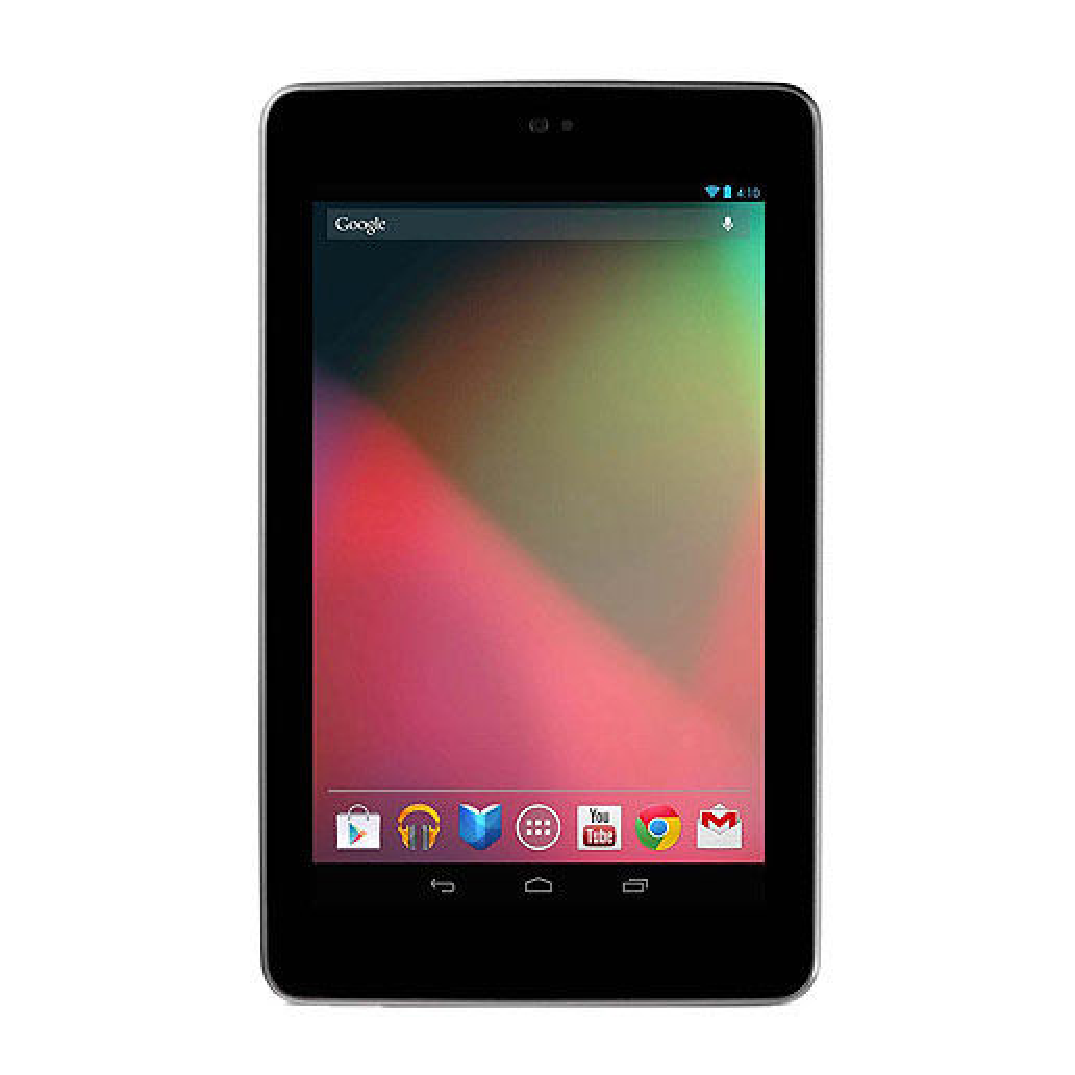
\includegraphics[width=.5\linewidth]{images/nexus7.eps}
  \end{center}
  \caption{Nexus 7}
  \label{fig:nexus7}
\end{figure}

\subsection{被験者}\label{ux88abux9a13ux8005}

被験者は大学生及び大学院生の計n名(男性x名, 女性y名,
平均zz歳)である(表\ref{table:tester})。

\begin{longtable}[c]{@{}lrr@{}}
\caption{被験者属性 \label{table:tester}}\tabularnewline
\toprule
被験者ID & 性別 & 年齢\tabularnewline
\midrule
\endfirsthead
\toprule
被験者ID & 性別 & 年齢\tabularnewline
\midrule
\endhead
A & 男 & 26\tabularnewline
B & 男 & 23\tabularnewline
C & 男 & 19\tabularnewline
\bottomrule
\end{longtable}

\subsection{実験タスク}\label{ux5b9fux9a13ux30bfux30b9ux30af}

タスク(課題)は5問用意した。

アプリケーションはフォアグラウンドの状態で、画面を見てもらっている状態でタスクを実行してもらった。

タスク達成時間は、アプリケーションがプログラムからの指示を受け取った時間を開始時間、
人が実行結果を返した時間を終了時間とし、アプリケーションに組み込んだ計測プログラムによって計測した。

タスクの教示方法 条件1
今から実行するプログラムは、コンピュータと人間を同じリソースとして扱えるプログラミング環境で実行されています。
このデバイスに、プログラムからの指示が来るので、それに対して、自分が正しいと思う値を返してください。

\subsection{実験手順}\label{ux5b9fux9a13ux624bux9806}

実験は、2014年12月25日に、慶應義塾大学SFCのデルタS112にて被験者1名ずつで行った(画像)。
被験者には実験用デバイスを手渡し、デバイスに表示される指示に対して、入力を行ってもらうタスク5問を行った。

実験終了後、実行時間や観察内容を元に、インタビューを行った。

\subsection{被験者インタビュー}\label{ux88abux9a13ux8005ux30a4ux30f3ux30bfux30d3ux30e5ux30fc}

実験後、被験者に対して半構造的インタビューを行った。
質問事項を図\ref{table:interview}に示す。

Table: インタビュー内容 \label{table:interview}

\begin{center}\rule{0.5\linewidth}{\linethickness}\end{center}

問1 コンピュータと同じ、処理を実行する立場と言われた時、どう思いますか
問2
自分や他人の感性判断をプログラムに組み込むことについて、どう思いますか
問3 返り値のフォーマット指定は 必要でしたか?
考えの幅が狭まるといったことはありますか?
扱いづらいものはありましたか? 問4
好きなキャラや俳優などからの指示のように見えるインタフェースだった場合、
動きに変化があると思いますか? 問5
命令元の人によって、指示に従うかどうかは変わりますか?

\subsection{実験結果}\label{ux5b9fux9a13ux7d50ux679c}

\subsubsection{反応速度}\label{ux53cdux5fdcux901fux5ea6}

\subsubsection{インタビュー}\label{ux30a4ux30f3ux30bfux30d3ux30e5ux30fc}

\section{性能評価実験}\label{ux6027ux80fdux8a55ux4fa1ux5b9fux9a13}

\subsection{実験趣旨}\label{ux5b9fux9a13ux8da3ux65e8-1}

\ref{sec:user-evaluation}節の実験によって、人間による処理の実行速度を計測した。
本節では、システムの通信部分における速度の計測を行う。

\subsection{実験装置}\label{ux5b9fux9a13ux88c5ux7f6e-1}
